\documentclass[12pt]{article}

\usepackage{geometry}
\usepackage{fancyhdr}
\usepackage{titlesec}
\usepackage{setspace}
\usepackage{dirtree}
\usepackage{xcolor}
\usepackage{graphicx}
\usepackage{url}

\PassOptionsToPackage{hyphens}{url}\usepackage{hyperref}

\setlength{\headheight}{15pt}

\geometry{a4paper, margin=3cm}
\titleformat{\section}{\large\bfseries}{\thesection}{1em}{}
\pagestyle{fancy}
\fancyhf{}
\rhead{Zesen Zhuang}
\lhead{Project-2 Report}
\rfoot{Page \thepage}

\begin{document}

\begin{titlepage}
    \centering
    \vfill
    {\bfseries\Large
        Project-2 Report\par
    }
    \vfill
    Submitted by:\\
    Zesen Zhuang\\
    zz229\\
    \vfill
    Date: \today
    \vfill
\end{titlepage}

\onehalfspacing

\section{Overview}

The following directory tree shows the structure of the project.

\dirtree{%
    .1 .
    .2 app.py \DTcomment{flask app for recommendation service and frontend with webui}.
    .2 docker/ \DTcomment{dockerfiles for images}.
    .3 api.dockerfile.
    .3 ml.dockerfile.
    .2 figures/ \DTcomment{images produced by tests}.
    .3 modify\_replica\_num.png.
    .3 update\_code.png.
    .3 update\_data.png.
    .2 generate\_model.py.
    .2 k8s/ \DTcomment{k8s yaml. I use Kustomize}.
    .3 base/.
    .4 config.properties \DTcomment{training data url and data version stored}.
    .4 config.properties.bak.
    .4 deployment.yaml \DTcomment{recommendation api and ui}.
    .4 kustomization.yaml.
    .4 pod.yaml \DTcomment{machine learning container}.
    .4 pvc.yaml \DTcomment{persistent volume claim}.
    .4 service.yaml.
    .2 makefile \DTcomment{automate the build, deploy and test}.
    .2 model.py \DTcomment{ml model source code}.
    .2 requirements.txt.
    .2 result/ \DTcomment{logs produced by tests}.
    .3 modify\_replica\_num.json.
    .3 status\_changes.txt.
    .3 update\_code.json.
    .3 update\_data.json.
    .2 static/ \DTcomment{flask ui static folder}.
    .3 css/.
    .4 styles.css.
    .2 templates/ \DTcomment{flask ui template folder}.
    .3 index.html.
    .3 recommendation.html.
    .2 test/ \DTcomment{api performance test}.
    .3 test\_api\_health.py.
    .2 visualization\_code/ \DTcomment{code to visualize test logs}.
    .3 plot.py.
}

\paragraph{GitHub Repo}
The GitHub repository is \url{https://github.com/Crinstaniev/cs401/tree/master/project-2/code}

\paragraph{Kustomize}
I applied \texttt{kustomize} to simplify the deployment.

\paragraph{UI}
I implemented a webui for the recommendation system and deployed in the api deployment.

\paragraph{GitHub Webhook to ArgoCD}
I configured a webhook in GitHub to trigger ArgoCD to sync the repository. Originally, ArgoCD will sync the repository every 3 minutes. Instead, I configured a webhook to trigger ArgoCD to sync the repository immediately.

\paragraph{PostSync Hook on Pod and Deployment Configuration}
Instead of manually changing the name of resources, I added ArgoCD hook to force the re-deployment of pods once any of the manifest file updates.

\section{Tests}

Three tests are conducted in this project. The first test is to change the replica number of \texttt{api} deployment. The second test is to change the code version (update the docker image) of \texttt{api} deployment. The third test is to change the data source of \texttt{ml} pod. The test results are shown in the following sections.

\subsection{Test: Change Replicas Number}

\begin{itemize}
    \item \textbf{Test Description:} Change the number of replicas from 1 to 5. I change the number of replicas in \texttt{deployment.yaml} from 1 to 5.
    \item \textbf{Test Result:} The test passed, ArgoCD detected the change pods number of \texttt{api} deployment to 5.
    \item \textbf{Test Analysis:} The test passed because the number of replicas can be changed. The service status during the test is shown in Figure \ref{fig:modify_replica_num}. It takes 5 seconds for the service to fully restart and increase the replica number.
\end{itemize}

\begin{figure}[!htbp]
    \centering
    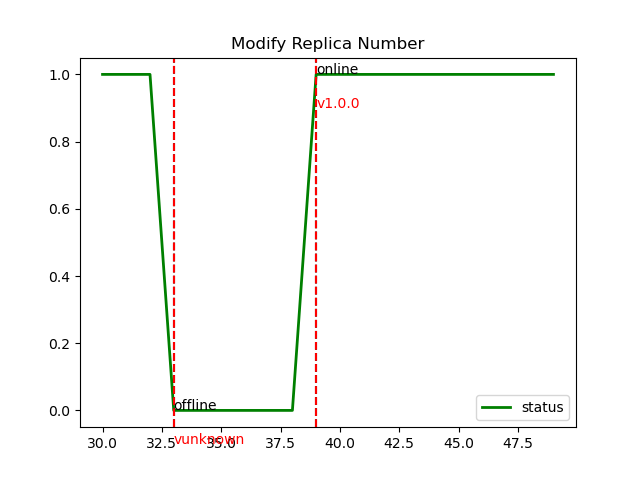
\includegraphics[width=.75\textwidth]{../code/figures/modify_replica_num.png}
    \caption{Service Status for Test: Change Replicas Number}
    \label{fig:modify_replica_num}
    \medskip
    \small
    The timeline is is trimmed. At time 0, the commit is pushed to GitHub and the webhook is triggered. Within few seconds, ArgoCD syncs the repository. Before 33 seconds, the deployment stayed at the old version. At 33, the service is down and resumes at 38.
\end{figure}

\subsection{Test: Code Update}

\begin{itemize}
    \item \textbf{Test Description:} I modified the health check API \texttt{/api/health} so that it return \texttt{\{ status: online! \}} instead of \texttt{\{ status: online \}} when the service is online.
    \item \textbf{Test Result:} The test passed, ArgoCD detected the change and re-deploy the deployment.
    \item \textbf{Test Analysis:} The service status during the test is shown in Figure \ref{fig:update_code}. Compared to test 1, it takes longer to reboot since the replica number increased to 5. After going online again, the service experienced a short-period down for which the reason worth further discussion.
\end{itemize}

\begin{figure}[!htbp]
    \centering
    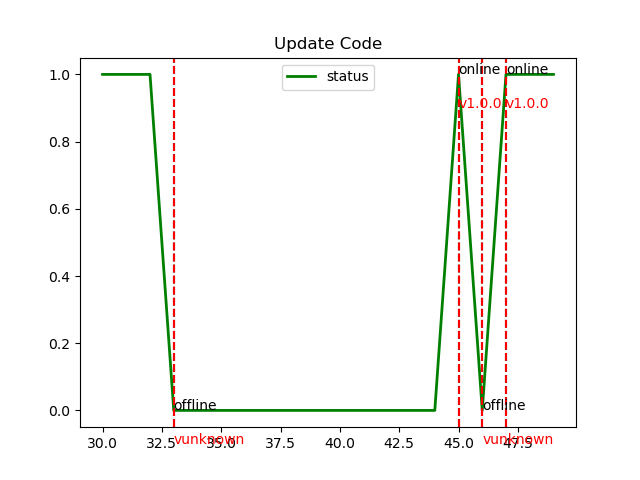
\includegraphics[width=.75\textwidth]{../code/figures/update_code.png}
    \caption{Service Status for Test: Update Code}
    \label{fig:update_code}
    \medskip
    \small
    The service went offline at 33 and back to online at 45. However, it was down again at 46 and went back immidiately at 47.
\end{figure}

\subsection{Test: Update Training Data}

\begin{itemize}
    \item \textbf{Test Description:} I changed the training data source from\\ \texttt{playlist-sample-ds1.csv} to \texttt{playlist-sample-ds2.csv}, and bump the data version in \texttt{config.properties} from \texttt{1.0.0} to \texttt{2.0.0}.
    \item \textbf{Test Result:} The test passed, ArgoCD detected the change and re-deploy the pod.
    \item \textbf{Test Analysis:} The service status during the test is shown in Figure \ref{fig:update_data}. Similar to test 2, it takes longer to reboot since the replica number is 5. The data version also bumpped to \texttt{v2.0.0} as the service went online again.
\end{itemize}

\begin{figure}[!htbp]
    \centering
    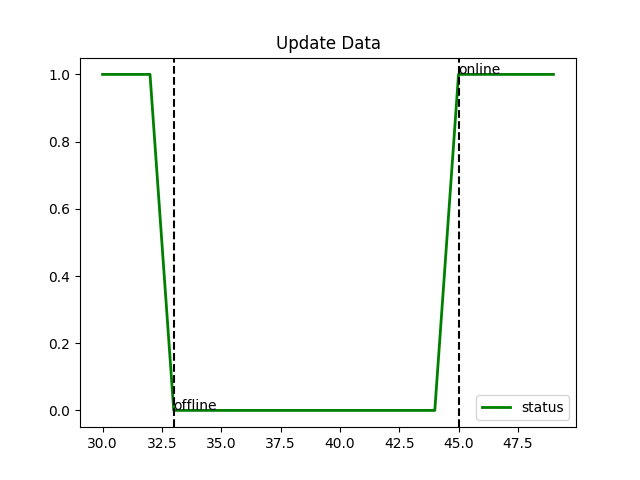
\includegraphics[width=.75\textwidth]{../code/figures/update_data.png}
    \caption{Service Status for Test: Update Data}
    \label{fig:update_data}
    \medskip
    \small
    The service went offline at 33 and back to online at 45.
\end{figure}

\end{document}
